\documentclass[12]{article}

\usepackage[margin=2.5cm]{geometry}
\usepackage{graphicx}
\usepackage[none]{hyphenat}
\usepackage{float}
\usepackage[nottoc, notlot, notlof]{tocbibind}
\usepackage{fancyhdr}
\pagestyle{fancy}
\fancyhead{}
\fancyfoot{}
\fancyhead[L]{\slshape\MakeUppercase{Predictive Sentiment Analysis}}
\fancyhead[R]{\slshape {Vera Rykalina}} 
\fancyfoot[C]{\thepage}
\parindent 0ex
%\setlength{\parskip}{2em}
\renewcommand{\baselinestretch}{2}
\begin{document}

\begin{titlepage}
\begin{center}
\vspace*{1cm}
\Large{\textbf{\MakeUppercase {Report}}}\\[3mm]
\Large{\textbf{Alert Analytics}}\\
\Large{\textbf{Helio}}\\
\vfill
\line(1,0){400}\\[5mm]
\Large{\textbf{\MakeUppercase{Predictive Sentiment Analysis}}}\\ [1mm]
\line(1,0){400}\\[2mm]
\vfill
By Vera Rykalina\\
September 16, 2020\\
\end{center}
\end{titlepage}
\tableofcontents
\thispagestyle{empty}
\clearpage
\setcounter{page}{1}

\section{Overview}
\subsection{What is  a sentiment analyisis?}
Sentiment analysis (SA) in plain English is the analysis of people's feelings such as attitudes, emotions, and opinions. It is a very vital tool that analyzes texts for polarity, from positive to negative. The SA prediction allows businesses to identify customer sentiment toward products, brands or services in online feedback.
\subsection{Client}
Helio is a smart phone and tablet app developer. It is working with a government health agency to create a suite of smart phone medical apps for use by aid workers in developing countries. This suite of apps will enable the aid workers to manage local health conditions by facilitating communication with medical professionals located elsewhere (one of the apps, for example, enables specialists in communicable diseases to diagnose conditions by examining images and other patient data uploaded by local aid workers). The government agency requires that the app suite be bundled with one model of smart phone.
\subsection{Objectives}
\textbf{Helio's Goal}\\
To determine which handset model from the list of five devices will bebundled with the suite of smart phone medical apps for use by aid workers indeveloping countries.\\
\textbf{Alert Analytics's Goal}\\
To help Helio narrow their list down to one device and provide them with a report that contains an analysis of sentiment toward the target devices, as well as a description of the methods and processes we used to arrive at our conclusions.

\section{Methodology}
\subsection{Approach}
There are a number of ways to capture sentiment from text documents. The approach we applied implies counting words associated with sentiment toward five preselected devices within relevant documents on the web. To discover patterns in the documents, we utilized the data and machine learning methods, allowing us to label each of these documents with a value that represents the level of positive or negative sentiment toward each of these devices. We then analyzed and compared the frequency and distribution of the sentiment for each of these devices.
\subsection{AWS and Common Crawl}
In order to really gauge the sentiment toward these devices, we performed the analysis on a very large scale. We used the cloud computing platform provided by Amazon Web Services (AWS) to conduct the analysis. The data sets we analyzed came from Common Crawl. Common Crawl is an open repository of web crawl data (over 5 billion pages so far) that is stored on Amazon’s Public Data Sets. Using AWS, we collected and developed a data matrix (large matrix) in the range of 20 thousand instances of relevant web documents from the Common Crawl.
\subsection{Predictive sentiment: small matrixes}
Helio provided us with the small data matrixes, including manually labelled subset of documents with a sentiment rating. We used this matrixes to develop machine learning models in R capable of determining web page sentiment automatically. 
\subsection{Predictive sentiment: large matrix}
We applied our models to the large matrix we collected using the AWS to understand the sentiment scores individually for iPhone and Galaxy. Lastly we analyzed this large predicted data and reported descriptive statistics to the client on the level of sentiment toward the handsets.

\section{Findings}
\subsection{Modelling}
We applied an objective numerical technique, the Recursive feature elimination (RFE), to the both iPhone and Galaxy small matrixes to reduce the number of features and select those with sensible contributions to the respective modelling. At least five algorithms were used for the machine learning:

\begin{itemize}
\item C5.0
\item Random Forest (RF)
\item Support Vector Machines (SVM)
\item Weighted k-Nearest Neighbors (KKNN)
\item Extreme Gradient Boosting (XGB)
\end{itemize}

All five classifiers were trained and optimized by "tuning" the associated  parameters. Optimal parameters were used to compare performances of the models. The performance metrics for iPhone and Galaxy are summarized in Table \ref{tab:Comp1} and Table \ref{tab:Comp2} respectively.
\\ 
\begin{table}[H]
\center
\begin{tabular}{c c c c c c}
\hline 
Algorithm & C5.0 & RF & SVM & KKNN & XGB \\ 
\hline \hline
Accuracy &  0.7686375 & 0.7429306 & 0.7236504 &  0.3359897 & 0.7874036\\ 
Kappa & 0.5484076 & 0.4815073 & 0.4486903 & 0.1635177 & 0.5918368\\ 
\hline
\end{tabular} 
\caption{Comparison of algorithm performance for iPhone}
\label{tab:Comp1}
\end{table}

\begin{table}[H]
\center
\begin{tabular}{c c c c c c}
\hline 
Algorithm & C5.0 & RF & SVM & KKNN & XGB \\ 
\hline \hline
Accuracy &  0.7942916 & 0.7680638 & 0.7459501 &  0.3301620 & 0.7971201\\ 
Kappa & 0.5918646 & 0.5203958 & 0.4686751 & 0.1783035 & 0.5951309\\ 
\hline
\end{tabular} 
\caption{Comparison of algorithm performance for Galaxy}
\label{tab:Comp2}
\end{table}

With 19 and 26 variables for iPhone and Galaxy respectively (according to RFE analysis) our models had fairly low accuracy to predict 6 categorical levels of sentiment. Nevertheless, XGB was chosen as an optimal model based on the comparative analysis. This model was utilized to work further on the predictive sentiment analysis task.
\newpage
\subsection{Analysis of review categories}
Deeper analysis of data allowed us to find out that our train data sets did not have enough and equal amount of information about each sentiment class to predict 6 class levels. The illustration of the disproportion of the data in relation to the review category for each small datasets is shown in Figure \ref{fig:imbA} for iPhone and in Figure \ref{fig:imbB} for Galaxy. 

\begin{figure}[H]
\centering
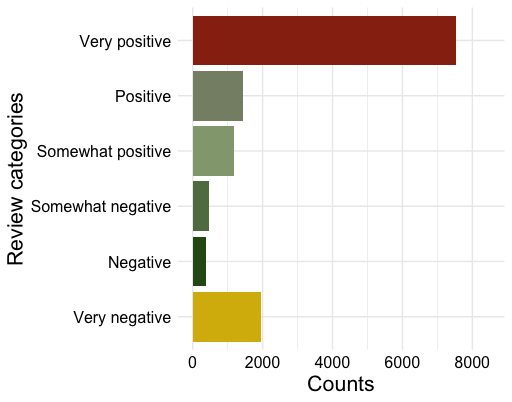
\includegraphics[scale=0.5]{imbA.png}
\centering
\caption{Data disproportion in relation to the review category for iPhone}
\label{fig:imbA}
\end{figure}


\begin{figure}[H]
\centering
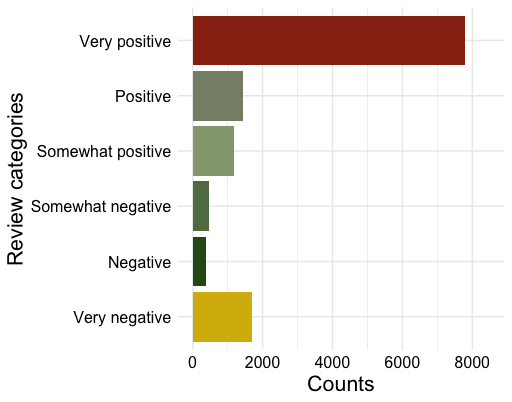
\includegraphics[scale=0.5]{imbB.png}
\centering
\caption{Data disproportion in relation to the review category for Galaxy}
\label{fig:imbB}
\end{figure}


\newpage
\subsection{Prediction}
The imbalance among the sentiment rating in the small matrixes was solved by decreasing the class levels of our dependent variable to only two categories: Negative and Positive. With implementation of the latter approach we reached more accurate models as it is illustrated in Table \ref{tab:Comp3}.

\begin{table}[H]
\center
\begin{tabular}{c c c c c c}
\hline 
Handset & Accuracy & Kappa \\ 
\hline \hline
iPhone &  0.883232 & 0.5775509 \\ 
Galaxy & 0.9040436 & 0.6313974 \\ 
\hline
\end{tabular} 
\caption{Performance of models with two review categories}
\label{tab:Comp3}
\end{table}

The result of our prediction is visualized in Figure \ref{fig:pred}. It is indeed a close call when we compare the two leading platforms, Apple iPhone and Samsung Galaxy head to head. The rapid technological development of each model of these brands is improving their performance, camera, and display. The ratios of positive and negative sentiments for both models are almost equal.

\begin{figure}[H]
\centering
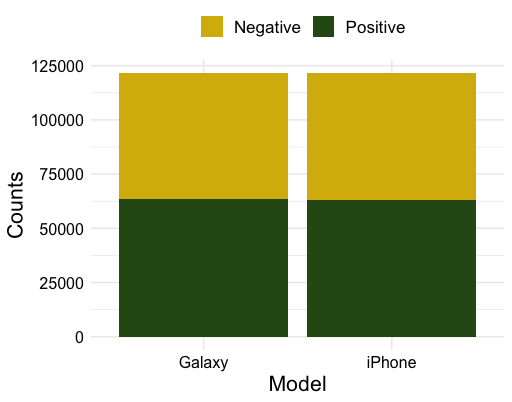
\includegraphics[scale=0.5]{pred.png}
\centering
\caption{Prediction of sentiments using two-class review}
\label{fig:pred}
\end{figure}



\section{Confidence}
Reducing the categories of review from six to two classes allowed us to achieve better accuracy and predict the sentiment towards iPhone and Galaxy. However, in our particular case of the imbalanced data the accuracy is not a correct metric. To understand to what extent we can trust our predictions, we considered the Sensitivity or Recall estimation. The Recal metric proved that overal prediction score for our models is about 50\% for both smartphone handsets. Although this is not an exellent overall result, we can rely on this prediction for our target class. 

With application of reduction in review categories, we generated better results. However, we assume that it can be possible to further improve the accuracy and kappa scores. Several steps could be taken in this direction. First, we can try to apply upsampling and downsampling techniques to balance the data. Second, we can try to decrease "noise" by removing features linked with the ios and google android operating systems. Indeed, words "iphone" and "samsunggalaxy" are not important  for our models as they only reflect how many times the handsets were mentioned in the webpages. 
Third, removing rows i.e. webpages with a small number of reviews for both datasets, is likely to provided us with more reliable infromation.


\section{Implications}
Our models predicted almost equal sentiments for the both leading smartphones. In relation to a final model selection, this result might be not that helpful for our client. However, additional analysis of the field should simplify the situation. As both platforms have similar amount of positive reviews, we could recommend a model which is easy of access on the market - Samsung Galaxy. 

\end{document}